% main.tex
% !TeX program = lualatex
% !BIB program = biber

\documentclass[12pt,letterpaper]{report}

\usepackage[spanish,es-nodecimaldot]{babel}
\usepackage{csquotes}
%referencias bib
\usepackage[
  backend=biber,
  style=verbose-trad2,    % notas al pie completas + 'Ibíd.' / 'Op. cit.'
  autocite=footnote,      % \autocite => nota al pie
  ibidtracker=context,    % controla cuándo usar Ibíd.
  pagetracker=true
]{biblatex}
\addbibresource{referencias.bib}

\usepackage{icontec_style}
\usepackage[hidelinks]{hyperref}

%Ajustes de cleveref
\usepackage[spanish,noabbrev,nameinlink]{cleveref}

%Configuraciones extra para referencias al español
\DefineBibliographyStrings{spanish}{references = {Referencias},}
\DefineBibliographyStrings{spanish}{
  ibidem = {Ibíd.},
  opcit  = {Op.\addabbrvspace cit.},
}

\usepackage[hang,flushmargin]{footmisc}
\renewcommand{\footnotelayout}{\setstretch{1}}

% Metadatos portada:
\icontecsetup{
  universidad = {Universidad Industrial de Santander},
  facultad    = {Facultad de Ingenierías Fisicomecánicas},
  programa    = {Escuela de Ingeniería de Sistemas e Informática},
  titulo      = {PROTOTIPO DE UN VIDEOJUEGO SERIO SOBRE SISTEMAS FERROVIARIOS EN COLOMBIA},
  autores     = {\\Miguel Ángel Plata Rodríguez -- 2190050\\Mateo Salazar Serrano -- 2200135},
  director    = {\\Urbano Eliécer Gómez Prada, PhD},
  ciudad      = {Bucaramanga},
  anio        = {\textit{(poner fecha de entrega)}}
}

\begin{document}

% Portada
\maketitleicontec

%Agradecimientos / Resumen / Abstract
% \chapter*{Agradecimientos}\addcontentsline{toc}{chapter}{Agradecimientos}
% \begin{resumen} ... \keywords{...} \end{resumen}
% \begin{abstractES} ... \keywords{...} \end{abstractES}

% Índices
\tableofcontents
\listoffigures
\listoftables
\clearpage

% ===== Contenido =====
% !TeX root = ../main.tex

\chapter{Introducción}

El transporte ferroviario ha desempeñado un papel fundamental en el desarrollo económico y logístico de los países industrializados. Colombia, a pesar de haber sido pionera en la introducción del ferrocarril en América Latina, ha experimentado un estancamiento significativo durante las últimas décadas, producto de la priorización de la infraestructura vial y de debilidades institucionales y técnicas en el sector. Según datos del Ministerio de Transporte, más del 60\% de la red ferroviaria nacional se encuentra inactiva, y el modo férreo apenas representa el 0,1\% de la carga nacional movilizada\autocite{mintransporteDatosCarga} .

Frente a este escenario, y en un momento de renovado interés evidenciado por proyectos como el corredor de La Dorada–Chiriguaná \autocite{mintransporteAPP2025} y el Regiotram de Bogotá \autocite{bogotaRegiotram2025} , el país se enfrenta no solo a retos técnicos y económicos, sino también a un desafío cultural y educativo: la limitada comprensión y valoración social del sistema ferroviario. 

La falta de conocimiento público sobre su funcionamiento, beneficios y complejidades ha contribuido históricamente a su baja priorización dentro de las políticas nacionales de transporte.

En este contexto, surge la necesidad de desarrollar herramientas innovadoras que no solo transmitan información, sino que logren despertar interés y promover la comprensión profunda de los desafíos que implica el desarrollo ferroviario. Una alternativa prometedora para lograrlo es la aplicación de tecnologías interactivas, en particular los videojuegos educativos, que combinan elementos lúdicos y pedagógicos para facilitar el aprendizaje experiencial. Bajo este paradigma, el Game-Based Learning (GBL) se postula como una estrategia educativa eficaz, utilizando entornos interactivos y dinámicos para promover la adquisición de conocimientos mediante la experiencia y la realimentacion \autocite{gblFrameworkExamining} .

Por su parte, los videojuegos serios, desarrollados con fines que trascienden el entretenimiento \autocite{seriousGamesMechanisms} , constituyen una herramienta idónea para representar de manera didáctica y accesible problemas complejos del mundo real, como los que enfrenta la infraestructura férrea colombiana.

Este trabajo de grado tiene como objetivo el desarrollo de un prototipo de videojuego serio orientado a la comprensión de los desafíos asociados al desarrollo ferroviario en Colombia. Implementado mediante el motor gráfico Unity 6 y el software de modelado Blender, y haciendo uso de la metodología Kanban, se busca crear una experiencia educativa que incorpore los criterios esenciales del GBL: inmersión, interacción, control del aprendiz, apoyo al aprendizaje, narrativa y evaluación \autocite{gblFrameworkExamining} .

\section{Planteamiento y justificación del problema}
Colombia, a pesar de haber sido pionera en la introducción del ferrocarril en Latinoamérica, se ha visto estancada en su desarrollo ferroviario. Tras una búsqueda en la plataforma web de la Agencia Nacional de Infraestructuras sobre los proyectos activos \autocite{aniProyectos}, de los 133 proyectos activos, sólo 4 son proyectos ferroviarios, de los cuales 2 llevan desde 1998 y 1999 en operación. Además, según datos del Ministerio de transporte de Colombia \autocite{mintransporteSurcos2024}, el 63,2\% de la red ferroviaria nacional se encuentra inactiva y, excluyendo el transporte de carbón y petróleo, el modo ferroviario apenas representa el 0,1\% de la carga nacional movilizada, lo cual evidencia una falta de interés e iniciativa por parte de los gobiernos que, a su vez, ha derivado en una priorización de la inversión pública en la infraestructura de carreteras \autocite{mintransporteDatosCarga}.

Según la monografía \textit{Desafíos del transporte ferroviario de carga en Colombia}, la dificultad en desarrollar efectivamente un transporte ferroviario en Colombia es debido a factores como los conflictos políticos, el manejo de los recursos y de la debilidad ingenieril del sector. Específicamente se menciona: “La institucionalidad del sector presenta hoy debilidades en materia de planeación y política ferroviaria; ingeniería ferroviaria conceptual…” \autocite[p.~17]{iabdDesafios}.

Actualmente, hay que considerar que recientemente la nación está intentando reiniciar el desarrollo de infraestructuras ferroviarias. Algunos de los proyectos que evidencian este reciente interés son: la firma del contrato de concesión, la primera Asociación Público-Privada (APP) del país, correspondiente al corredor de La Dorada–Chiriguaná \autocite{mintransporteAPP2025}; el inicio de las obras del Regiotram de Occidente, que beneficiará a Bogotá y a sus municipios aledaños \autocite{bogotaRegiotram2025}; y el megaproyecto del Tren de Cercanías del Valle del Cauca \autocite{valoraTrenValle2024}, que busca conectar Cali con Jamundí, Yumbo y Palmira.

Aun así, ante la carencia de herramientas que refuercen la planeación y la ingeniería ferroviaria, resulta oportuno desarrollar recursos que impulsen el aprendizaje y la concientización sobre los desafíos de este sector.

Los videojuegos en su mayoría se enfocan en el entretenimiento del jugador, sin embargo, existe la posibilidad de diseñar juegos educativos, tal es el caso de un estudio descrito en el artículo “Examining the characteristics of game-based learning: A content analysis and design framework” \autocite{gblFrameworkExamining} en donde, a partir del análisis y la codificación de 194 artículos diferentes sobre juegos educativos, se definió un marco de diseño de un \textit{Game-Based Learning} (GBL), o aprendizaje basado en un juego.

Un GBL se compone por dos grupos de características, las primarias y secundarias, siendo las primarias los aspectos que se consideran esenciales para un juego educativo \autocite{gblFrameworkExamining}: Criterios de inmersión, interacción, control del aprendiz, apoyo al aprendizaje, narrativa y evaluación.

Además, según el libro \textit{Serious Games: Mechanisms and Effects}, se define un videojuego serio como “cualquier forma de software de juego interactivo basado en computadora (…) y que se ha desarrollado con la intención de ser más que entretenimiento.” \autocite[p.~6]{seriousGamesMechanisms}. Aspecto que aplica para el caso de estudio de este proyecto, ya que se tiene planteado, además de entretener, educar sobre los desafíos del desarrollo ferroviario en Colombia.

Al respecto, existen diversos antecedentes de videojuegos de simulación enfocados en diseñar y construir sistemas férreos, como son el \textit{Railway Empire} \autocite{railwayEmpire} ambientado en Estados Unidos entre siglo XIX y XX, \textit{Railroad Tycoon 3} \autocite{railroadTycoon3} basado en escenarios para recrear sistemas férreos importantes en la historia de la humanidad y \textit{Train Valley 2} \autocite{trainValley2} enfocado en la resolución de puzles; sin embargo, ninguno de los videojuegos mencionados tiene propósitos más allá del entretenimiento, objetivo que sí se busca en este proyecto de grado.

Tras una búsqueda con el motor Google Academics y usando la ecuación: (“Colombia” AND “Sistema Férreo” AND (“Videojuego Serio” OR “Videojuego de simulación” OR “Videojuego educativo”)), se encontró solamente una tesis de grado que tenía como objetivo “Investigar sobre interfaces hápticas para aplicaciones 3D, así como analizar su interactividad y usabilidad en una aplicación interactiva para la maqueta de transportes ESPOCH.” \autocite{tesisInterfacesHapticas}, en el que no es un aspecto suficiente para que sea considerado el desarrollo de un videojuego serio, ya que en ningún momento describe el proceso de desarrollo de un videojuego, solo se menciona como un ejemplo. En ese orden de ideas, se puede concluir que no se encontró ningún videojuego serio de sistemas ferroviarios ambientado en Colombia.

Por lo anterior, se formula la siguiente pregunta de investigación:

\textbf{¿Cuál debería ser la estructura de un prototipo de videojuego serio sobre los desafíos del desarrollo del sistema ferroviario en Colombia y cómo se implementaría para que tenga en cuenta los criterios de inmersión, interacción, control del aprendiz, apoyo al aprendizaje, narrativa y evaluación del marco GBL?}

En el orden de ideas de lo manifestado, se puede considerar viable una iniciativa en el desarrollo de un prototipo de software para la educación del sector ferroviario, por lo tanto, se propone implementar un primer prototipo de un videojuego serio de sistemas ferroviarios en Colombia, con el fin de concientizar la comprensión de algunos de los desafíos que conllevaría la planeación y el desarrollo de la infraestructura férrea en el país.

Se espera que el prototipo del videojuego serio sobre los desafíos del sistema ferroviario en Colombia incorpore las características primarias del marco GBL como la evaluación (cómo se mide el aprendizaje), la inmersión (cuán envolvente es el entorno del juego), la interacción (cómo se comunica el jugador con el juego o entre jugadores), el control del aprendiz (el grado de autonomía que tiene el usuario), el apoyo al aprendizaje (tutoriales y ayudas) y la narrativa (la historia o contexto que da sentido a la experiencia). Estas características se usarán para “ayudar a trazar rutas de aprendizaje más personalizadas, motivadoras y potencialmente efectivas para el aprendizaje.” \autocite[p.~10]{gblHandbook2019}.

El prototipo tendrá una prueba piloto dirigida a estudiantes UIS, con el objetivo de evaluar la experiencia del jugador y el desempeño del software. La prueba se orientará a determinar si el prototipo resulta agradable en su uso y se encuentre libre de errores, permitiendo identificar áreas de mejora para quienes deseen dar continuidad a este proyecto.

\newpage
\section{Objetivos}

\subsection{Objetivo General}
Desarrollar un prototipo de un videojuego serio para la comprensión de algunos de los desafíos que conllevaría el mejoramiento de la infraestructura férrea en Colombia, usando GBL, Unity 6, Blender y RUP adaptada con elementos de Kanban.

\subsection{Objetivos Específicos}
\begin{enumerate}[label=\arabic*.]
  \item Definir las historias de usuario del videojuego serio a partir del marco GBL para el apoyo de la comprensión de algunos de los desafíos del desarrollo férreo.
  \item Diseñar los componentes que integran el videojuego serio tales como los sistemas de evaluación, inmersión, interacción y control del jugador a partir del contexto de sistemas ferroviarios en Colombia.
  \item Implementar el videojuego serio integrando un sistema interactivo de un mapa 3D, así como eventos ambientales, económicos y sociales usando Unity 6 y Blender.
  \item Evaluar el videojuego serio realizando pruebas de funcionalidad y usabilidad.
\end{enumerate}

% !TeX root = ../main.tex

\chapter{Marco de referencia}

\section{Sistemas Ferroviarios en Colombia}

Aunque Colombia fue pionera en introducir el sistema ferroviario en Latinoamérica, el desarrollo de este presentó diversos declives, abandonos y una mala gestión por parte del estado. En consecuencia, el modo carretero fue ganando poder consolidándose como la principal forma de transporte tanto de carga como de pasajeros en Colombia \autocite{iabdDesafios}. Para entender los desafíos actuales del sistema ferroviario colombiano, es importante analizar su historia, su avance y los retos que hoy en día enfrenta.

\subsection{Historia}

Históricamente, los ferrocarriles en Colombia surgieron a finales del siglo XIX, principalmente como concesiones privadas. En 1954, se intentó unificar las distintas líneas existentes bajo una sola entidad estatal, los Ferrocarriles Nacionales de Colombia (FNC). La red alcanzó su máxima extensión en 1961 con 3{,}431 km. Sin embargo, el desarrollo de las carreteras y una gestión considerada débil llevaron al abandono progresivo de muchos trazados. Tras la liquidación de la FNC en 1991 y un intento posterior con Ferrovías que tampoco cumplió las expectativas, se optó por concesionar los corredores con mayor potencial: la Red Férrea del Atlántico (1999) y la Red Férrea del Pacífico (1998) \autocite{iabdDesafios}.

Según la monografía \textit{Desafíos del transporte ferroviario de carga en Colombia} \autocite{iabdDesafios}, los ferrocarriles en Colombia se introdujeron a finales del siglo XIX tras acuerdos con concesiones privadas, pero en 1954, como un intento de unificar todas las líneas ferroviarias de trocha angosta (914 mm) en una sola entidad estatal, se fundó los Ferrocarriles Nacionales de Colombia (FNC). Este fue el primero de muchos intentos que, durante 50 años, ninguno llegó a cumplir las expectativas.

\subsection{Dominio del transporte por carretera}

Hoy en día, la red ferroviaria nacional cuenta con una longitud total estimada en 3{,}533 km \autocite{ponencia337_2023} y evidencia una importante subutilización, ya que se reveló en un informe de una ponencia para el segundo debate del proyecto de ley número 337 del 2023 \autocite{ponencia337_2023} en donde dice que el 63\% (2.262 km) de las vías del país están inactivos. Así mismo, se muestra que en los últimos 10 años el transporte de carga por carretera pasó de un 70.8\% en el 2011 a un 85.5\% en el 2021. En las \cref{fig:grafica1_modo_carretero,fig:grafica2_modo_ferroviario} se muestran datos directos del Ministerio de Transporte actualizado al 2023 sobre el transporte de carga en modo carretero vs modo férreo:

\begin{figure}[H]\centering
  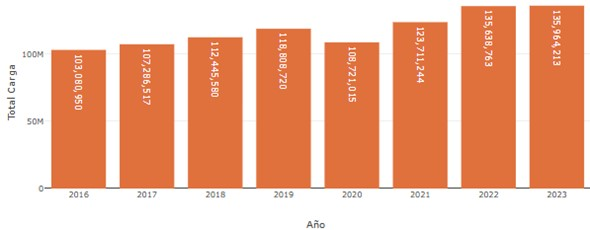
\includegraphics[width=\linewidth]{figures/grafica1_modo_carretero.jpg}
  \caption{Gráfica 1. Movimiento de carga -- Modo Carretero. Fuente: \autocite{mintransporteDatosCarga}.}
  \label{fig:grafica1_modo_carretero}
\end{figure}

\begin{figure}[H]\centering
  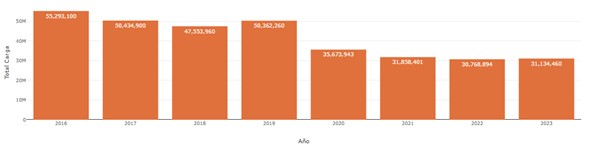
\includegraphics[width=\linewidth]{figures/grafica2_modo_ferroviario.jpg}
  \caption{Gráfica 2. Movimiento de carga -- Modo Ferroviario. Fuente: \autocite{mintransporteDatosCarga}.}
  \label{fig:grafica2_modo_ferroviario}
\end{figure}

Así mismo, el Ministerio de Transporte revela que el transporte de pasajeros en modo férreo es muy despreciable en comparación con el transporte por carretera, por ejemplo, en el 2023 se movilizaron casi 90 millones de pasajeros por carretera versus los casi 500 mil en tren \autocite{mintransporteDatosCarga}.

\section{Game-Based Learning}

El aprendizaje basado en juegos, o Game-Based Learning (GBL) por sus siglas en inglés, es una metodología educativa que hace uso de juegos, tanto digitales como analógicos, como herramienta principal para la enseñanza y el aprendizaje. Dichos juegos están diseñados con el objetivo de mejorar la motivación, la participación y el aprendizaje de quienes buscan aprender un tema especifico \autocite{gblHandbook2019}. Cabe señalar que el GBL no es lo mismo que la gamificación, ya que este introduce elementos de juegos en contextos donde normalmente estos no son la norma. Por otro lado, el GBL utiliza juegos específicamente creados con el objetivo de facilitar el aprendizaje de contenidos y habilidades.

Múltiples estudios sugieren que los juegos, en sus diversas formas, pueden motivar e interesar a los estudiantes, aumentar la retención del material y mejorar las habilidades de razonamiento y el pensamiento complejo \autocite{gblBeneficios}. Además, el GBL ofrece un entorno de aprendizaje donde los errores no tienen consecuencias reales, lo que permite a los estudiantes experimentar, explorar y aprender de sus fallos, y hay que entender que, dentro del contexto de los videojuegos, el fracaso funciona como una forma de retroalimentación, donde el fallo no es el final, sino una enseñanza de los errores cometidos.

Diseñar un GBL requiere la integración de características tales como: Criterios de inmersión, interacción, control del aprendiz, apoyo al aprendizaje, narrativa y evaluación \autocite{gblFrameworkExamining}:

\begin{enumerate}
  \item \textbf{Criterios de inmersión:} Estos criterios comprenden el diseño tanto visual como sonoro para ambientar al jugador; el diseño visual incluye elementos como la apariencia general del juego y sus personajes, así como la forma de representación de la información clave; el diseño sonoro proporciona sonidos de fondo que se utilizan a menudo para dirigir la atención del jugador a eventos o momentos importantes del juego, señalar la presencia de peligro u oportunidad, inducir emociones positivas o negativas, y reconocer el éxito o el fracaso de una tarea específica.
  \item \textbf{Criterios de interacción:} Los criterios de interacción son aquellos que se encargan de permitir al jugador interactuar con el entorno del juego, permitiéndole tomar decisiones y realizar acciones.
  \item \textbf{Control del aprendiz:} El control del aprendiz se trata del nivel de autonomía que se le da al jugador sobre cómo quiere afrontar los desafíos que le presenta el juego, un ejemplo de esto es la libertad de elección en juegos de toma de decisiones, donde la elección del jugador afecta la narrativa y desarrollo de la historia.
  \item \textbf{Apoyo del aprendizaje:} Se trata de los sistemas y herramientas que tiene el juego para guiar y reforzar el proceso de aprendizaje del jugador, ya sea con tutoriales, pistas, o recursos adicionales y explicaciones.
  \item \textbf{Narrativa:} La narrativa en un juego es la historia que se cuenta mientras el jugador participa. Esta historia puede incluir personajes, misiones, problemas por resolver y un contexto que da sentido a lo que se está haciendo. Una narrativa bien construida motiva al jugador a seguir jugando; una buena historia puede generar sentimientos o emociones, además de poder guiar a los jugadores en su toma de decisiones.
  \item \textbf{Evaluación:} La evaluación en los juegos permite registrar el progreso del jugador, medir su desempeño e identificar errores durante el desarrollo de la partida.
\end{enumerate}

\section{Motores gráficos y herramientas de modelado 3D}

Un motor gráfico es un sistema diseñado para el desarrollo de videojuegos y aplicaciones interactivas que requieren representación visual. Cuenta con herramientas para la creación y gestión de todas las características de un videojuego, como lo son la renderización 2D y 3D, motores de físicas, sistemas de sonido, soporte para compilación de código, entre otros.

Algunos ejemplos bastante conocidos de motores de videojuegos gratuitos son el Unreal Engine \autocite{unrealSite} y Unity \autocite{unitySite}, los cuales permiten que personas de todo el mundo puedan desarrollar sus propios proyectos digitales.

Unreal Engine “permite crear juegos y experiencias con un alto nivel de detalle geométrico gracias al sistema de geometría de micro poligonal virtualizada de Nanite y a los mapas de sombras virtuales” \autocite{unrealFeaturesNanite} y ha sido utilizado en producciones de alto nivel, no solo en la industria de los videojuegos, sino también en el cine y la arquitectura, un ejemplo de esto es en la serie de \textit{The Mandalorian} donde “parte de esta serie fue rodada en un set de producción virtual con tecnología Unreal Engine” \autocite{mandalorianMeristation2022} gracias a su capacidad para generar entornos visuales realistas. Unity, por otro lado, cuenta con una amplia comunidad de usuarios, una amplia accesibilidad, y tiene la capacidad de exportar proyectos a más de 25 plataformas diferentes \autocite{unitySite}. Además, es especialmente popular en el desarrollo de juegos móviles, simulaciones y experiencias en realidad aumentada (AR) y realidad virtual (VR), siendo utilizado en proyectos como \textit{Hollow Knight}, \textit{Escape From Tarkov}, \textit{Genshin Impact} y diversas aplicaciones educativas y médicas como \textit{Virtual Reality Surgical Simulation Suite} (VR3S) \autocite{vr3s}.

Por otro lado, una herramienta de modelado es un software diseñado para crear, manipular y modificar modelos tanto bidimensionales (2D) como tridimensionales (3D) de objetos y escenas. Entre las herramientas de modelado 3D más populares se encuentran Blender \autocite{blenderSite}, el cual es un software gratuito y de código abierto; Autodesk Maya \autocite{mayaSite}, utilizado mayormente en la industria de los efectos especiales, el cine y la animación; y 3ds Max \autocite{maxSite}, usado mayormente en diseño arquitectónico y visualización de productos.

\subsection{Unity}

Unity es una plataforma utilizada para “crear y hacer crecer juegos y experiencias interactivas en todas las principales plataformas, desde móviles, PC y consolas, hasta realidad extendida (XR)” \autocite{unityCompany}, haciendo uso de los lenguajes de programación C\# y .NET.

Esto es posible ya que Unity es un motor multiplataforma que permite desarrollar aplicaciones para múltiples dispositivos simultáneamente, sin la necesidad de hacer grandes modificaciones en el código. Cuenta también con una comunidad de usuarios bastante activa donde los usuarios comparten conocimientos, recursos y activos en múltiples redes sociales, así como también en sus foros oficiales. Ciertamente, Unity cuenta con su propia tienda en línea, la Unity Asset Store, donde los desarrolladores pueden comprar y vender activos y herramientas. Entre estos activos se encuentran modelos 3D, plantillas para la creación de juegos, herramientas de desarrollo, entre otros elementos útiles.

Además, cuenta con múltiples licencias de uso, cuyo precio varía dependiendo de necesidades de los estudios, sin embargo, también cuenta con licencias gratuitas para uso personal, estudiantes, y pequeñas organizaciones con ingresos y fondos recaudados en los últimos 12 meses menor a \$200K USD \autocite{unityPricing}.

\subsection{Blender}

Blender es una herramienta de modelado de código abierto y gratuito usado para la creación de gráficos y animaciones en 2D y 3D, la cual “cuenta con una amplia variedad de herramientas que lo hacen adecuado para casi cualquier tipo de producción de medios. Las personas y estudios de todo el mundo lo utilizan para proyectos de hobby, comerciales y películas” \autocite{blenderManual282}.

Blender puede ser utilizado para múltiples propósitos, ya sea el modelado de objetos, la animación mediante sus herramientas de \textit{rigging} y líneas de tiempo, el texturizado, el renderizado gracias a los sistemas EEVEE y Cycles, la edición de video, la composición digital o incluso los efectos visuales (VFX).

Además, Blender cuenta con la Licencia Pública General GNU (GPL) \autocite{blenderAbout}, lo que permite que el público pueda descargar, modificar y distribuir el programa con total libertad cuantas veces necesite.

\section{Modelos de desarrollo}

En la ingeniería de software existen diferentes metodologías que fueron diseñadas con el objetivo de establecer un marco de trabajo a la hora de construir un proyecto. En 1970, el ingeniero de software Winston W. Royce estableció por primera vez el modelo en cascada \autocite{cataldi1999} o también conocido como modelo tradicional, en él se propone un enfoque secuencial en donde cada fase depende del anterior, comenzando desde la fase de análisis hasta terminar con la fase de pruebas \autocite{pressman2001}. No obstante, este modelo es poco utilizado en la actualidad debido a su falta de realismo; plantea un desarrollo de software de forma estrictamente lineal, sin contemplar ajustes ni retroalimentación por parte del cliente durante el proceso.

En consecuencia, en el 2001 un grupo de 17 ingenieros escribieron y firmaron el “Manifiesto por el Desarrollo Ágil de Software” \autocite{agileManifesto2001}, donde se encuentran los 12 principios que se deben cumplir a la hora de construir software de manera ágil. En resumen, la agilidad en la que se refiere el manifiesto es la capacidad del equipo de adaptarse a cambios, incluso si estos son pedidos en las últimas etapas del desarrollo, ya que el objetivo principal es realizar varias entregas constantes en ciclos de trabajo definidos con una retroalimentación para satisfacer lo más posible al cliente.

\subsection{RUP}

El Proceso Racional Unificado o RUP (por sus siglas en inglés de Rational Unified Process), es una metodología ágil de desarrollo de software creado por la empresa Rational, que más adelante fue adquirido por IBM \autocite{ibmAcquiresRational2002}. RUP no fue descrita como una metodología con pasos estrictamente detallados, sino más bien, como un conjunto de declaraciones sobre lo que se debería reflejar durante el desarrollo del software, esto con el fin de que pueda ser flexible y adaptable según las necesidades del proyecto.

RUP, en realidad, es una extensión de una anterior metodología llamada UP, la cual propuso 4 fases \autocite{anderson2003}:

\begin{enumerate}
  \item \textbf{Inicio:} Es una fase corta donde se desarrolla la idea inicial del proyecto; se identifica el modelo de negocio y sus riesgos, y se provee un boceto de la estructura a partir de unos objetivos generales. Es muy importante que los requerimientos que se detallen aquí no deben restringir la flexibilidad o soluciones que el equipo de trabajo podría encontrar después.
  \item \textbf{Elaboración:} En esta fase se comienza a detallar los requerimientos, historias de usuario, casos de uso, entre otros diagramas según las necesidades del proyecto. Se sigue teniendo en cuenta la flexibilidad del equipo para mitigar los mayores riesgos. Normalmente, durante el desarrollo de esta fase se requieren más iteraciones que el anterior.
  \item \textbf{Construcción:} Es la fase más larga del proyecto, ya que es donde se empieza a programar el software; se escribe, testea y depura el código. En cada iteración se debe cumplir con algún entregable funcional y normalmente se prioriza las funciones más importantes del software.
  \item \textbf{Transición:} En esta última fase, sucede la entrega del proyecto al cliente y se empieza el mantenimiento a largo plazo, esto también incluye documentación de usuario (manual de uso), preparación del entorno o incluso entrenamiento del usuario. Es muy probable que se tenga que realizar cambios a partir de la retroalimentación de los usuarios finales y así continuamente lanzar nuevas versiones.
\end{enumerate}

\begin{figure}[H]\centering
  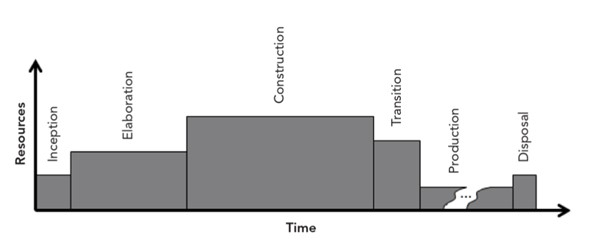
\includegraphics[width=\linewidth]{figures/fig3_rup_tiempo_vs_recursos.jpg}
  \caption{Fig 3. Tiempo vs recursos utilizados en cada fase en RUP. Fuente: \autocite[p.~296]{anderson2003}.}
  \label{fig:fig3_rup_tiempo_vs_recursos}
\end{figure}

Junto con las fases, IBM también introduce los \textit{artifacts} que se traduce como “artefactos” \autocite{anderson2003}. Estos son simplemente los resultados que se generan durante el transcurso del proyecto o también se les considera los entregables y pueden ser entre documentación, modelos o elementos de un modelo.

\subsection{Kanban}

Kanban se traduce del japonés como “tarjeta de señal”, ya que esta metodología fue en un principio creada en la década de los 40 por la empresa Toyota para la organización de inventario. Sin embargo, en el mundo de la ingeniería de software y gracias a David J. Anderson \autocite{anderson2003}, se empezó a utilizar como una metodología de seguimiento de desarrollo y control de roles.

Existe toda una filosofía detallada detrás que no se abordará, sino precisamente, en su aplicación directa. Como bien su nombre dice, se trata de tarjetas virtuales o físicas donde se representa un sistema de gestión de proceso visual en un tablero, donde cada tarjeta representa una tarea asignada a un miembro de un equipo. Estas tarjetas viajan de izquierda a derecha pasando por columnas que indican el estado de la tarea. Es común indicar las columnas como “To do” (Por hacer), “In progress” (En progreso) y “Done” (Terminado), pero esto no es realmente estricto en Kanban y es flexible según las necesidades del proyecto o del hito a alcanzar.

Cada tarjeta forma parte de un objetivo en común y se suele aplicar en iteraciones con fechas de entrega detalladas, es por esto por lo que este sistema de gestión es muy común adaptarlas junto con otras metodologías ágiles para desarrollo de software.

Las tarjetas se componen de un título, una breve descripción, el nombre de la persona asignada, la fecha de creación y la fecha de entrega; estos componentes, como se ha repetido en el documento, nunca son estrictas y se pueden agregar más o menos detalles según sea el caso.

% !TeX root = ../main.tex


\chapter{Metodología}

La metodología que se utilizará es RUP simplificada y adaptada con tableros Kanban, por ello, se adecuaron los objetivos del proyecto de la sección 2 del documento a las fases descritas en RUP.

\section{Inicio}

En esta fase, aunque ya avanzada por la investigación hecha para las entregas del tema y el plan de trabajo de grado, se aborda todos los conceptos utilizados en el artículo recopilatorio GBL \autocite{gblFrameworkExamining}. El objetivo de esta fase es definir un primer documento de historias de usuario y riesgos del prototipo, identificar los requisitos clave (funcionalidades GBL, desafíos ferroviarios a representar) a alto nivel. Las actividades son las siguientes:

\begin{enumerate}
  \item \textbf{Definir las HU:} Se define un primer documento borrador de las historias de usuario iniciales del videojuego para que puedan cumplir con los requisitos para ser un GBL.
  \item \textbf{Identificar riesgos:} Se definen en una lista las posibles dificultades técnicas encontradas en Unity para cumplir con las historias de usuario planteadas.
  \item \textbf{Planificar la fase de elaboración:} Se empieza a elaborar un primer borrador del documento de los requisitos clave funcionales.
\end{enumerate}

\section{Elaboración}

El objetivo de esta fase es mitigar los riesgos principales, agrupar y jerarquizar las HU, y definir y validar la arquitectura base del videojuego. Las actividades son las siguientes:

\begin{enumerate}
  \item \textbf{Organizar las HU:} Se pule el documento de las historias de usuario previamente encontradas y se organizan en épicas para después definir un orden de prioridades. Además, se explicará cómo se abordarán los criterios del GBL y los desafíos ferroviarios en las historias de usuario.
  \item \textbf{Elaborar maqueta:} Se construye una primera maqueta en Unity atacando directamente a la lista de identificación de riesgos, se obtiene un primer “esqueleto” del juego sobre el cual se empezará la fase de construcción.
  \item \textbf{Refinar la lista de riesgos:} Se modifican los riesgos según el resultado de la primera maqueta, para después investigar posibles soluciones.
  \item \textbf{Planificar las iteraciones:} Se definen las iteraciones que se darán en la fase de construcción, priorizando los requerimientos e historias de usuario más importantes.
\end{enumerate}

\section{Implementación}

El objetivo de esta fase es construir el prototipo del videojuego de forma incremental, completando las funcionalidades y asegurando la calidad a través de pruebas continuas. La actividad principal de esta fase es implementar el videojuego y, a partir de las iteraciones planificadas, se empieza a construir el código en Unity apoyándose en el sistema de gestión de procesos Kanban. Para esto se asignarán los requerimientos e historias de usuario a cada uno de los miembros del equipo y se empezará a avanzar en un tablero Kanban como el siguiente:

\begin{table}[H]\centering
\caption{Tablero Kanban propuesto para la fase de Construcción.}
\label{tab:kanban-construccion}
\begin{tabular}{@{}lcccc@{}}
\toprule
\textbf{Equipo} & \textbf{Por hacer} & \textbf{Haciéndose} & \textbf{Revisándose} & \textbf{Hecho} \\
\midrule
Miguel & & & & \\
Mateo  & & & & \\
\bottomrule
\end{tabular}
\end{table}

La columna “Revisándose” hará que el integrante contrario revise su historia de usuario y, una vez este lo pruebe y le dé su aval, pasa a considerarse como “Hecho”.

\section{Evaluación}

El objetivo de esta fase es entregar el prototipo a los usuarios de la prueba piloto (estudiantes UIS) y escribir el libro final entregable del trabajo de grado. Las actividades son las siguientes:

\begin{enumerate}
  \item \textbf{Obtener y organizar grupo de prueba:} Se acuerda con un grupo de estudiantes UIS para acordar una fecha y lugar para realizar la prueba.
  \item \textbf{Obtener los resultados:} Una vez realizada la prueba se les realiza un pequeño cuestionario para evaluar el rendimiento, la usabilidad y las recomendaciones del jugador.
  \item \textbf{Preparar informe y presentación:} Recopilar la documentación, el proceso de trabajo y los resultados para agruparlos en un libro entregable junto con una presentación.
\end{enumerate}

% !TeX root = ../main.tex

\chapter{Resultados}

\section{Requerimientos}
% (Completar más adelante con el contenido de tu PDF si lo deseas)

\section{Diseño}
% (Completar)

\section{Implementación}
% (Completar)

\section{Pruebas}
% (Completar)
 

% Bibliografía
\printbibliography[title={Referencias}]

% (Opcional) Apéndices
% \appendix
% \include{appendices/apendice-a}

\end{document}
